% 本文件接续 sample_chapter_1.tex；各章的图、表和公式标签应保持唯一。
\xmuchapter{研究方法与结果排版示例}{Research Methods and Result Presentation}
\label{chap:sample-results}

\xmusection{参数估计方法}{Parameter Estimation Method}

本章以第\ref{chap:sample-background}章的线性模型为例，
演示方法说明、多行公式、分段函数、结果曲线、数据表格和算法的排版。
全部数值均为人为构造的示例数据\footnote{本章数据仅用于检查图表和公式的显示效果，不能作为实验结果使用。}。
文献引用沿用项目现有的参考文献条目，关于排版系统的介绍可参阅文献\cite{samplebook}。

\xmusubsection{最小二乘估计}{Least-Squares Estimation}

对于式\eqref{eq:sample-model}，定义预测值为 $\hat{y}_i = \hat{a}x_i + \hat{b}$。
通过最小化观测值与预测值之间的平方误差，可得到参数估计：
\begin{align}
    J(a,b) &= \sum_{i=1}^{N}\left[y_i-(ax_i+b)\right]^2,
    \label{eq:sample-objective} \\
    \hat{\boldsymbol{\theta}} &=
    \underset{\boldsymbol{\theta}}{\operatorname{arg\,min}}\,
    \left\|\mathbf{y}-\mathbf{X}\boldsymbol{\theta}\right\|_2^2.
    \label{eq:sample-estimate}
\end{align}
当式\eqref{eq:sample-design}中的矩阵 $\mathbf{X}$ 列满秩时，估计结果可写为
\begin{equation}
    \hat{\boldsymbol{\theta}} =
    \left(\mathbf{X}^{\mathrm{T}}\mathbf{X}\right)^{-1}
    \mathbf{X}^{\mathrm{T}}\mathbf{y}.
    \label{eq:sample-solution}
\end{equation}

\xmusubsection{评价指标与分段函数}{Evaluation Metrics and Piecewise Function}

以均方根误差衡量预测结果与观测结果的差异：
\begin{equation}
    E_{\mathrm{RMSE}} =
    \sqrt{\frac{1}{N}\sum_{i=1}^{N}\left(y_i-\hat{y}_i\right)^2}.
    \label{eq:sample-rmse}
\end{equation}
为演示分段函数，设定误差阈值 $\tau = 0.15$，并定义示例判定函数
\begin{equation}
    q(E) =
    \begin{cases}
        1, & 0 \leq E \leq \tau, \\
        0, & E > \tau.
    \end{cases}
    \label{eq:sample-criterion}
\end{equation}
其中，$q(E)=1$ 表示误差满足示例阈值。该阈值仅用于说明公式写法。

\xmusection{示例数据与结果分析}{Sample Data and Result Analysis}

\xmusubsection{数据表格}{Data Table}

取表\ref{tab:sample}中的参数，令输入量依次为 $0$、$1$、$2$、$3$ 和 $4$，
构造表\ref{tab:sample-results}中的观测数据。对应的估计参数为
$\hat{a}=2.0$、$\hat{b}=1.0$。

\begin{table}[htbp]
    \centering
    \caption{观测值、预测值与误差对比}
    \label{tab:sample-results}
    \floatunit{单位：无量纲}
    \begin{tabular}{ccccc}
        \toprule
        \tablehead{样本序号} & \tablehead{输入值 $x_i$} &
        \tablehead{观测值 $y_i$} & \tablehead{预测值 $\hat{y}_i$} &
        \tablehead{误差 $y_i-\hat{y}_i$} \\
        \midrule
        1 & 0 & 1.1 & 1.0 & $ 0.1$ \\
        2 & 1 & 2.9 & 3.0 & $-0.1$ \\
        3 & 2 & 5.0 & 5.0 & $ 0.0$ \\
        4 & 3 & 6.9 & 7.0 & $-0.1$ \\
        5 & 4 & 9.1 & 9.0 & $ 0.1$ \\
        \bottomrule
    \end{tabular}
    \floatnote{注：预测值由示例模型计算。资料来源：作者构造的示例数据。}
\end{table}

\xmusubsection{曲线绘制与图例}{Plotting Curves and Legends}

图\ref{fig:sample-results}使用模板已加载的绘图宏包，
直接根据表\ref{tab:sample-results}中的数据绘制散点与曲线，无需新增图片文件。
坐标轴和图例使用英文，图题及资料说明使用中文。

\begin{figure}[htbp]
    \centering
    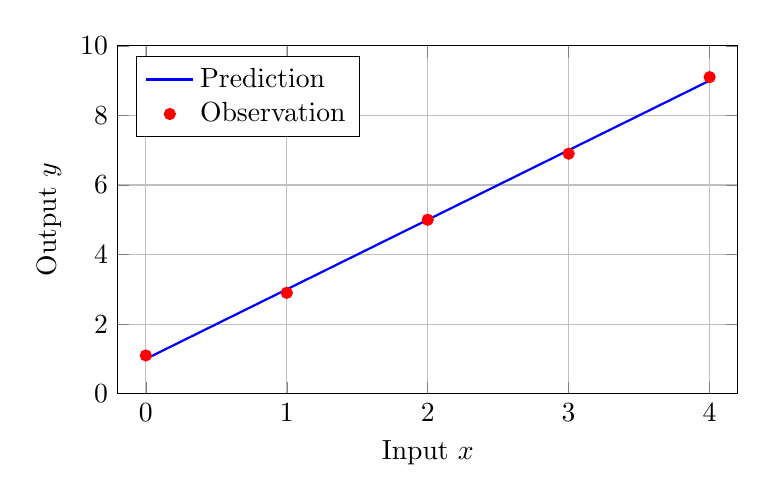
\begin{tikzpicture}
        \begin{axis}[
            width=0.78\textwidth,
            height=6cm,
            xlabel={Input $x$},
            ylabel={Output $y$},
            xmin=-0.2, xmax=4.2,
            ymin=0, ymax=10,
            xtick={0,1,2,3,4},
            grid=major,
            legend pos=north west,
            legend cell align=left
        ]
            \addplot[blue, thick, mark=none] coordinates {
                (0,1) (1,3) (2,5) (3,7) (4,9)
            };
            \addlegendentry{Prediction}
            \addplot[red, only marks, mark=*, mark size=2pt] coordinates {
                (0,1.1) (1,2.9) (2,5.0) (3,6.9) (4,9.1)
            };
            \addlegendentry{Observation}
        \end{axis}
    \end{tikzpicture}
    \caption{示例模型的观测值与预测结果}
    \label{fig:sample-results}
    \floatnote{资料来源：依据表\ref{tab:sample-results}中的示例数据绘制。}
\end{figure}

\subsubsection{误差分析}

将表\ref{tab:sample-results}中的数值代入式\eqref{eq:sample-rmse}，
可得 $E_{\mathrm{RMSE}}=\sqrt{0.008}\approx 0.0894$。
根据式\eqref{eq:sample-criterion}，有 $q(E_{\mathrm{RMSE}})=1$。
图表、公式和正文应采用一致的数据，正式写作时还应补充实验条件及误差来源分析。

\xmusection{算法排版示例}{Algorithm Typesetting}

以下伪代码使用模板已加载的算法环境，展示输入、输出、循环及条件语句的写法。
算法\ref{alg:sample-evaluation}对应前述误差计算和阈值判定过程。

\begin{algorithm}[htbp]
    \caption{示例模型的误差评价流程}
    \label{alg:sample-evaluation}
    \KwIn{观测值 $y_i$、预测值 $\hat{y}_i$、样本数量 $N$、阈值 $\tau$}
    \KwOut{均方根误差 $E_{\mathrm{RMSE}}$ 与判定结果 $q$}
    $S \leftarrow 0$\;
    \For{$i \leftarrow 1$ \KwTo $N$}{
        $S \leftarrow S + (y_i-\hat{y}_i)^2$\;
    }
    $E_{\mathrm{RMSE}} \leftarrow \sqrt{S/N}$\;
    \eIf{$E_{\mathrm{RMSE}} \leq \tau$}{
        $q \leftarrow 1$\;
    }{
        $q \leftarrow 0$\;
    }
\end{algorithm}

\xmusection{本章小结}{Chapter Summary}

本章通过示例数据展示了方法描述、公式推导、分段函数、结果表格、曲线图和算法。
结合第\ref{chap:sample-background}章，可观察同章与跨章引用的效果，
以及图、表和公式随章节自动编号的效果。
